\PassOptionsToPackage{dvipsnames}{xcolor}  % avoid options class with metropolis theme
\documentclass[aspectratio=169]{beamer} 


\usepackage{amsmath}
\usepackage{amsfonts}
\usepackage{graphicx}
\usepackage{ifthen}
\usepackage{mathtools}
\usepackage{bm}

\newcommand{\Ni}{\mathcal N(i)}
\newcommand{\deltamin}{\delta_{{\min}}}

\newcommand{\alphahat}{\hat{\alpha}}
\newcommand{\betahat}{\hat{\beta}}
\newcommand{\deltahat}{\hat{\delta}}
\newcommand \Omegap [1] {\Omega_P \left(#1\right)}

\newcommand{\gammahat}{\hat{\gamma}}

\newcommand{\Q}{Q}
\newcommand{\X}{X}
\newcommand{\Xhat}{\widehat{\X}}

\newcommand{\onevec}{\mathbf{1}}

\newcommand \calN {\mathcal{N}}

\newcommand{\sigmaeps}{\sigma_{\varepsilon}}

\newcommand \bigoh [1] {\mathcal O \paren*{#1}}
\newcommand \littleoh [1] {o \paren*{#1}}

\newcommand{\RDPG}{\operatorname{RDPG}}

\newcommand{\R}{\mathbb{R}}

\newcommand{\E}[2][]{%
	\ifthenelse{ \equal{#1}{} }
	{\ensuremath{\mathbb{E} \brac*{#2}}}
	{\ensuremath{\mathbb{E} \brac*{#2 \, \middle \vert \, #1}}}
}

\DeclarePairedDelimiter{\paren}{(}{)}
\DeclarePairedDelimiter{\brac}{[}{]}
\DeclarePairedDelimiter{\abs}{\lvert}{\rvert}
\DeclarePairedDelimiter{\norm}{\lVert}{\rVert}

\newcommand \diid {\stackrel{\mathrm{iid}}{\sim}}

\DeclareMathOperator*{\diag}{diag}
\DeclareMathOperator*{\supp}{supp}
\DeclareMathOperator*{\Bern}{Bern}

\usetheme[numbering=none, block=fill]{metropolis}
\setsansfont{Fira Sans}
\setmonofont{Fira Mono}

\usepackage{natbib}
\usepackage{nicematrix}
\usepackage{fontawesome5}

\newtheorem{proposition}{Proposition}
\newtheorem{assumption}{Assumption}
\theoremstyle{remark}
\newtheorem*{remark}{Remark}

\setbeamercolor{background canvas}{bg=white}
\setbeamercolor{normal text}{fg=black}
\setbeamercolor{frametitle}{bg=black, fg=white}

\hypersetup{colorlinks,allcolors=black}

\title{Understanding linear regression for social networks}
\date{August 7, 2025 @ Joint Statistical Meetings 2025}
\author{Alex Hayes}

\institute{Department of Statistics\\University of Wisconsin-Madison}

\begin{document}

\maketitle

\begin{frame}{Understanding social influence is fundamental in a highly connected society}
    
    \begin{columns}
        \begin{column}{0.35\textwidth}
            \centering
            \begin{tikzpicture}[scale=0.6]
                \node[shape=circle,fill=Mahogany] (A) at (0,1) {};
                \node[shape=circle,fill=gray,label=below left:{
\includegraphics[scale=0.2]{./figures/bacteria.png}}] (B) at (1,-1) {};
                \node[shape=circle,fill=Mahogany] (C) at (1.5,2.5) {};
                \node[shape=circle,fill=Mahogany] (D) at (2.75,0.5) {};
                \node[shape=circle,fill=gray,label=above right:{
\includegraphics[scale=0.2]{./figures/bacteria.png}}] (E) at (4.3,2.4) {};
                \node[shape=circle,fill=Mahogany,label=below:{
\includegraphics[scale=0.2]{./figures/bacteria.png}}] (F) at (3.4,-1.4) {};
                \node[shape=circle,fill=gray,label=right:{
\includegraphics[scale=0.2]{./figures/bacteria.png}}] (G) at (4.7,0.1) {};
                
                \draw (A) -- (B);
                \draw (A) -- (C);
                \draw (B) -- (C);
                \draw (B) -- (D) -- (F);
                \draw (C) -- (D) -- (E);
                \draw (B) -- (F) -- (G) -- (E) -- (C);
            \end{tikzpicture}
        \end{column}
        \begin{column}{0.65\textwidth}
            \vspace{6mm} \\
            \onslide<1->{
                \textbf{Direct effect}: if I get \textcolor{Mahogany}{vaccinated}, I am less likely to get sick 
\includegraphics[scale=0.2]{./figures/bacteria.png}
                \vspace{4mm} \\
                \textbf{Contagion}: if my friends get sick 
\includegraphics[scale=0.2]{./figures/bacteria.png}, I am more likely to get sick 
\includegraphics[scale=0.2]{./figures/bacteria.png}
                \vspace{4mm} \\
                \textbf{Interference}: if my friends get \textcolor{Mahogany}{vaccinated}, I am less likely to get sick 
\includegraphics[scale=0.2]{./figures/bacteria.png}
                \vspace{7mm} \\
            }
            \onslide<2->{
                \footnotesize * Can be defined counterfactually \citep{vazquez-bare2023}, but we do not consider counterfactual inference in this talk.
            }
        \end{column}
    \end{columns}
\end{frame}

\begin{frame}{This talk is about the \underline{linear-in-means} model}
    \textcolor{Mahogany}{Very popular} tool for estimating social influence \\
    \vspace{4mm}
    Used in education, crime, health, social policy, etc \footnote{\cite{sacerdote2001, epple2011, soetevent2007, trogdon2008, duflo2003, bertrand2000, glaeser1996, patacchini2012a, carrell2013}, etc} \\
    \vspace{4mm}
    I discovered an issue with this model
\end{frame}

\begin{frame}{\underline{Linear-in-means} models are a canonical tool to estimate social influence}
    \footnotesize
    \begin{table}[]
        \begin{tabular}{llcl@{\hspace{4em}}lcl}
            \onslide<1->{Outcome         & (sick?)       & $Y_i$    & $\in \{0, 1\}$           & Base rate                  & $\alpha$ & $\in \R$}      \\
            \onslide<2->{Node degree     & (num friends) & $d_i$    & $\in \{0, 1, 2, \dots\}$ & Contagion                  & $\beta$  & $\in (-1, 1)$} \\
            \onslide<2->{Edge $i \sim j$ & (friends?)    & $A_{ij}$ & $\in \{0, 1\}$}          & \onslide<3->{Direct effect & $\gamma$ & $\in \R$ }     \\
            \onslide<3->{Treatment       & (vaccinated?) & $T_i$    & $\in \{0, 1\}$ }         & \onslide<4->{Interference  & $\delta$ & $\in \R$}      \\
        \end{tabular}
    \end{table}
    \Large
    \vspace{4mm}
    \begin{equation*}
        \onslide<1->{
            \underbrace{Y_i}_\text{sick?} =
            \alpha
        }
        \onslide<2->{
            + \beta \underbrace{\frac{1}{d_i} \sum_{j \, : \, A_{ij} = 1} Y_j}_{\substack{\text{fraction} \\ \text{sick} \\ \text{friends}}}
        }
        \onslide<3->{
            + \gamma \underbrace{T_i}_\text{vaccinated?}
        }
        \onslide<4->{
            + \delta \underbrace{\frac{1}{d_i} \sum_{j \, : \, A_{ij} = 1} T_j}_{\substack{\text{fraction} \\ \text{vaccinated} \\ \text{friends}}}
        }
        \onslide<5-> {
            + \underbrace{\varepsilon_i}_\text{error}
        }
    \end{equation*}
    
    \onslide<6->{\footnotesize Letting $G = D^{-1} A$ be the row-normalized adjacency matrix, can write in matrix-vector form: \Large
        \begin{equation*} \label{eq:lim-mv}
            Y = \alpha 1_n + \beta G Y + T \gamma + G T \delta + \varepsilon
        \end{equation*}
    }
\end{frame}

\begin{frame}{Linear-in-means models are closely connected to spatial autoregression models}
    \centering
    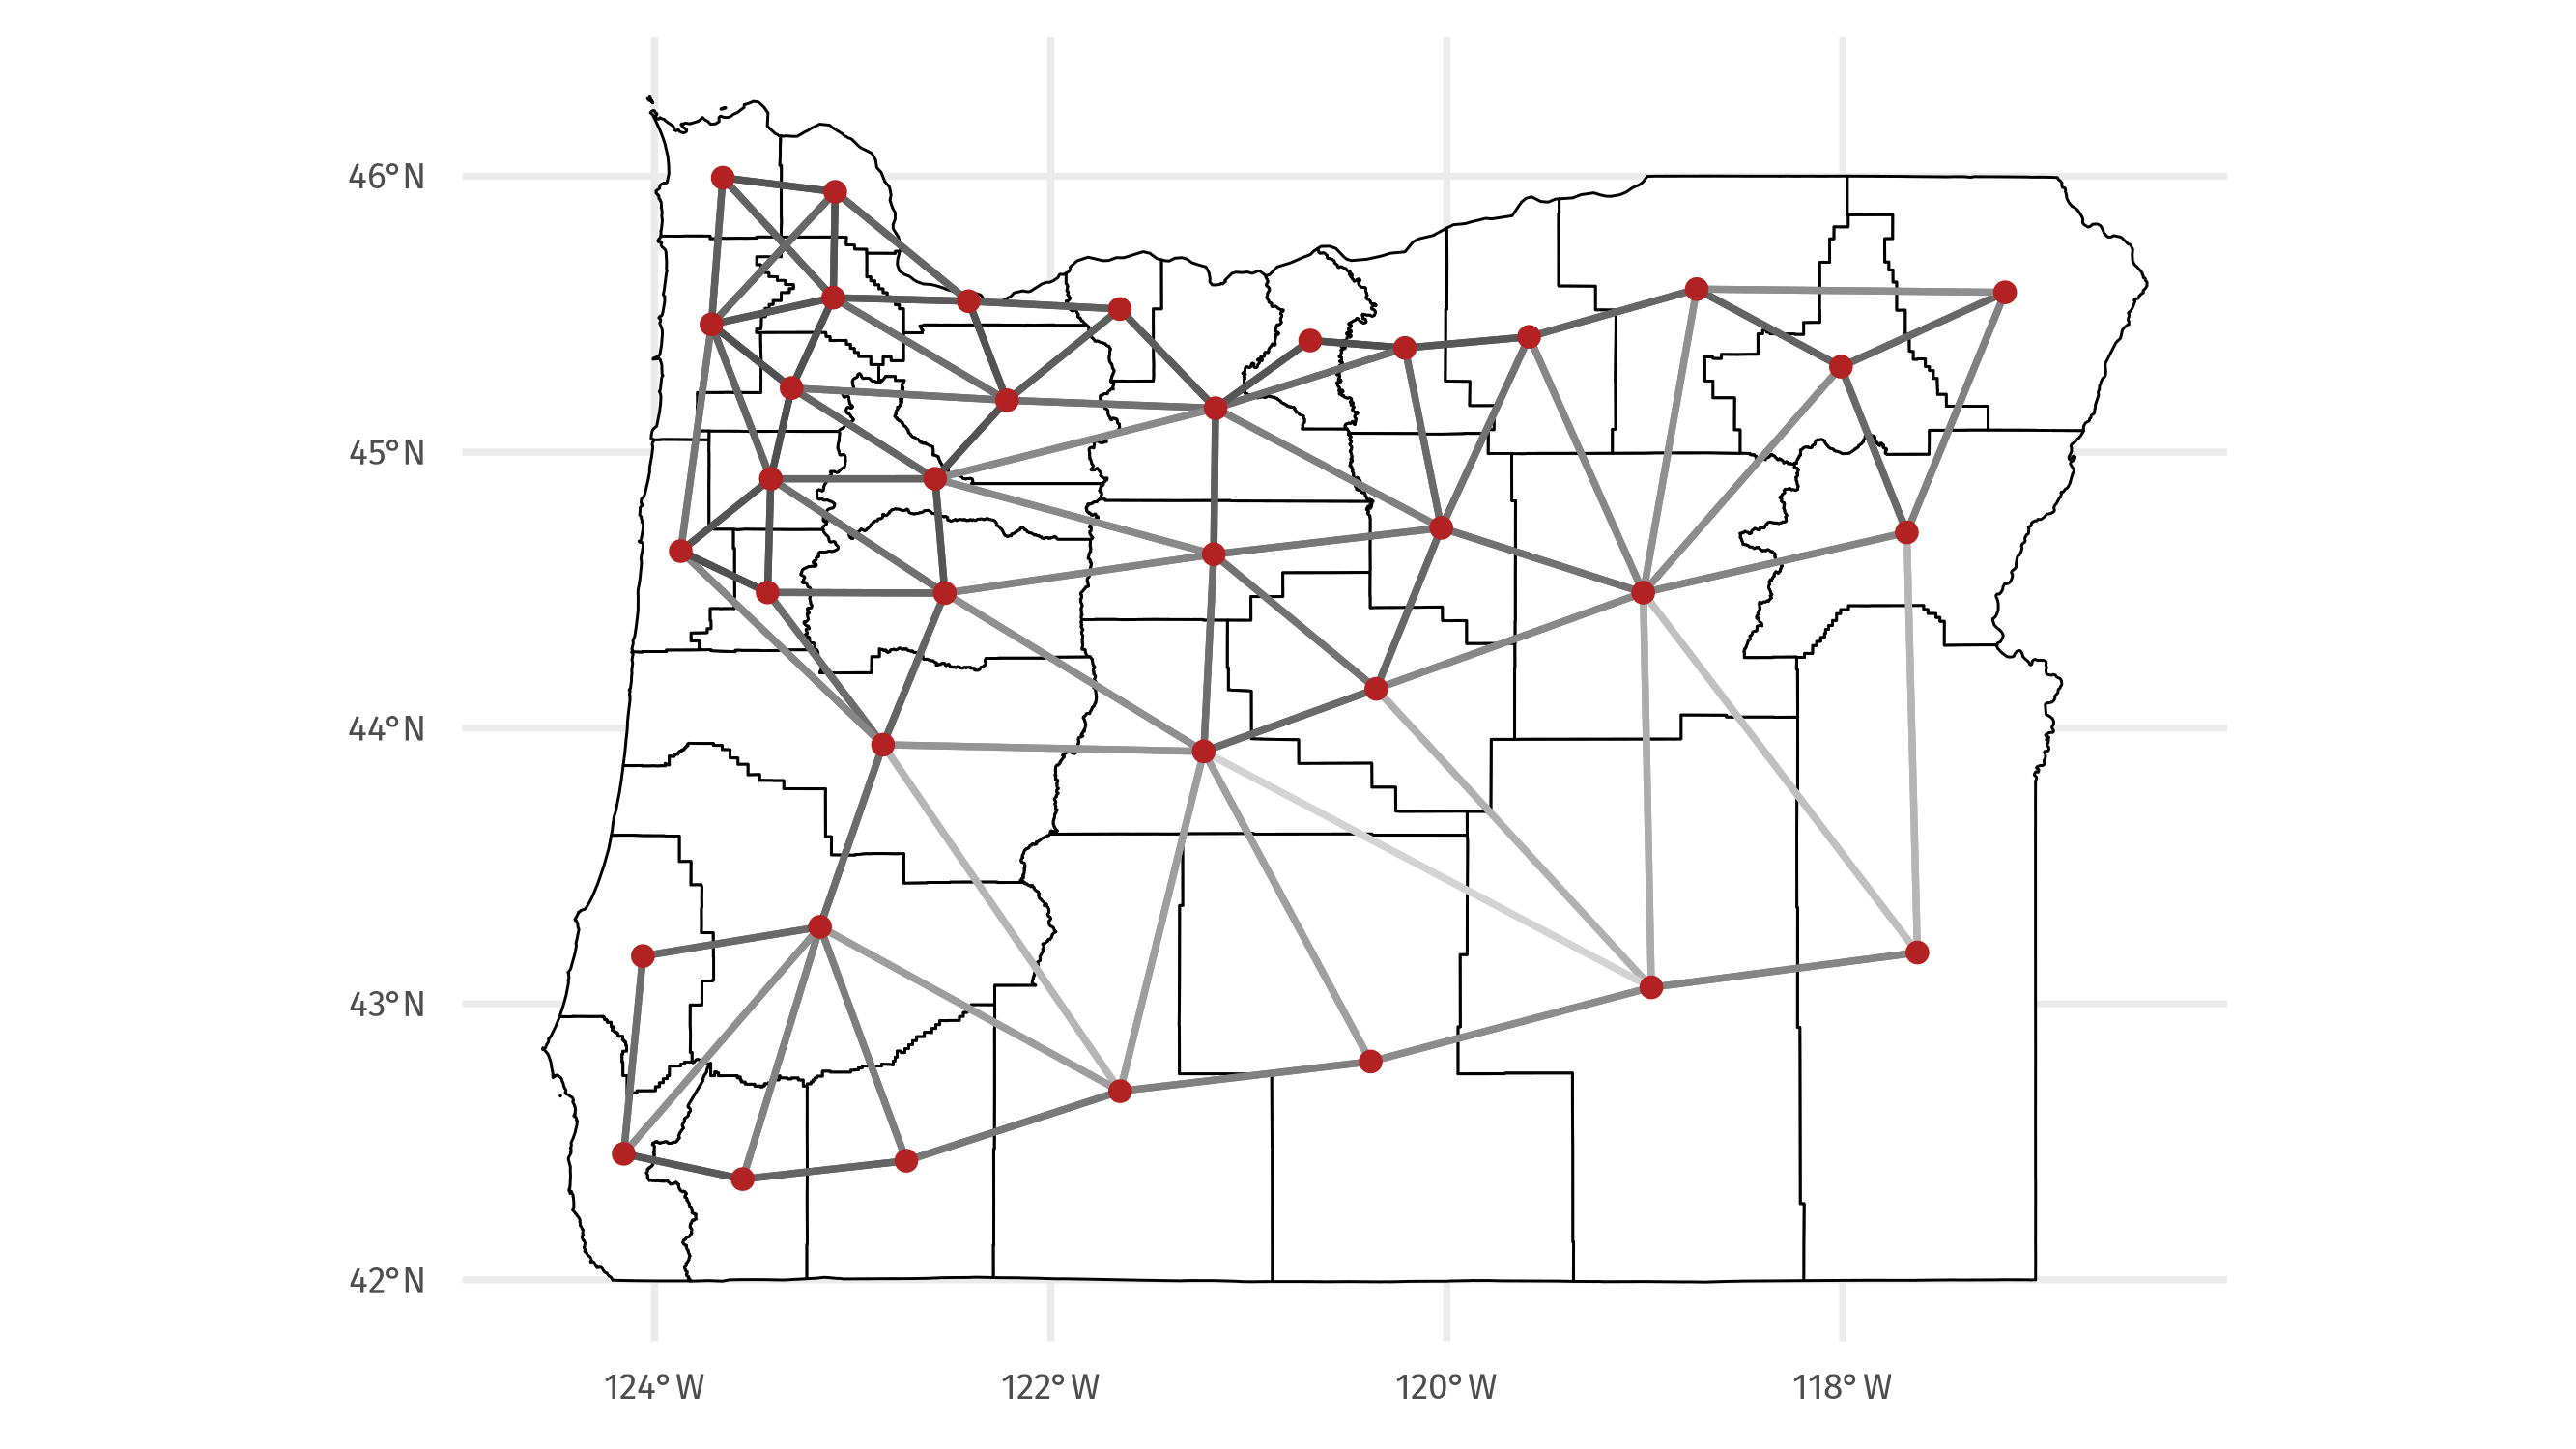
\includegraphics[height=0.95\textheight]{./figures/oregon_map.png}
\end{frame}

\begin{frame}{Identification in the linear-in-means model can be subtle}
    \centering
    
\includegraphics[height=0.95\textheight, page=2, trim={0 14cm 0 0}, clip]{./papers/manski.pdf}
\end{frame}


\begin{frame}{Linear-in-means models are famously suspectible to perfect collinearity}
    \begin{minipage}{0.49\textwidth}
        \centering
        \begin{tikzpicture}
            \node[shape=circle,fill=Mahogany,label=above left:{$T_1 = 1$}] (A) at (0,1) {};
            \node[shape=circle,fill=gray,label=below left:{$T_2 = 0$}] (B) at (1,0) {};
            \node[shape=circle,fill=Mahogany,label=above right:{$T_3 = 1$}] (C) at (1.5,1.5) {};
            \node[shape=circle,fill=Mahogany,label=above right:{$T_4 = 1$}] (D) at (2.75,0.5) {};
            
            \path (A) edge [loop above] node {} (A);
            \path (B) edge [loop below] node {} (B);
            \path (C) edge [loop above] node {} (C);
            \path (D) edge [loop above] node {} (D);
            
            \draw (A) -- (B);
            \draw (A) -- (C);
            \draw (A) -- (D);
            \draw (B) -- (C);
            \draw (B) -- (D);
            \draw (C) -- (D);
        \end{tikzpicture}
    \end{minipage}
    \begin{minipage}{0.49\textwidth}
        \centering
        \begin{tikzpicture}
            \node[shape=circle,fill=Mahogany,label=above left:{$[GT]_1 = 3/4$}] (A) at (0,1) {};
            \node[shape=circle,fill=gray,label=below left:{$[GT]_2 = 3/4$}] (B) at (1,0) {};
            \node[shape=circle,fill=Mahogany,label=above right:{$[GT]_3 = 3/4$}] (C) at (1.5,1.5) {};
            \node[shape=circle,fill=Mahogany,label=above right:{$[GT]_4 = 3/4$}] (D) at (2.75,0.5) {};
            
            \path (A) edge [loop above] node {} (A);
            \path (B) edge [loop below] node {} (B);
            \path (C) edge [loop above] node {} (C);
            \path (D) edge [loop above] node {} (D);
            
            \draw (A) -- (B);
            \draw (A) -- (C);
            \draw (A) -- (D);
            \draw (B) -- (C);
            \draw (B) -- (D);
            \draw (C) -- (D);
        \end{tikzpicture}
    \end{minipage}
    
    \begin{equation*}
        \begin{bmatrix}
            Y_1 \\
            Y_2 \\
            Y_3 \\
            Y_4
        \end{bmatrix}
        =
        \begin{bNiceMatrix}[first-row,first-col]
             & 1_n                     & GY   & T & GT                        \\
             & \textcolor{Mahogany}{1} & GY_1 & 1 & \textcolor{Mahogany}{3/4} \\
             & \textcolor{Mahogany}{1} & GY_2 & 0 & \textcolor{Mahogany}{3/4} \\
             & \textcolor{Mahogany}{1} & GY_3 & 1 & \textcolor{Mahogany}{3/4} \\
             & \textcolor{Mahogany}{1} & GY_4 & 1 & \textcolor{Mahogany}{3/4} \\
        \end{bNiceMatrix}
        \begin{bmatrix}
            \textcolor{Mahogany}{\alpha} \\
            \beta                        \\
            \gamma                       \\
            \textcolor{Mahogany}{\delta}
        \end{bmatrix}
        +
        \begin{bmatrix}
            \varepsilon_1 \\
            \varepsilon_2 \\
            \varepsilon_3 \\
            \varepsilon_4
        \end{bmatrix}
    \end{equation*}
    
    \centering
    Can't distinguish base rate $\textcolor{Mahogany}{\alpha}$ from interference $\textcolor{Mahogany}{\delta}$ due to collinearity
\end{frame}

\begin{frame}{It's widely believed that this ``reflection problem'' is rarely a problem in practice}
    
    \begin{proposition}[\citealt{bramoulle2009}]
        Suppose $\gamma \beta + \delta \neq 0$. If $I, G$ and $G^2$ are linearly independent, i.e., that $a I + b G + c G^2 = 0$ requires $a = b = c = 0$, then $\alpha, \beta, \gamma$ and $\delta$ are identified.
    \end{proposition}
    
    There is no perfect collinearity and peer influence is identified when there are \textcolor{Mahogany}{open triangles} (``intransitivity'') in the network
    \begin{columns}
        \begin{column}{0.5\textwidth}
            \centering
            \begin{tikzpicture}
                \node[shape=circle,fill=gray,label=above left:A] (A) at (0,1) {};
                \node[shape=circle,fill=Mahogany,label=below left:B] (B) at (1,0) {};
                \node[shape=circle,fill=Mahogany,label=above right:C] (C) at (1.5,1.5) {};
                \node[shape=circle,fill=Mahogany,label=above right:D] (D) at (2.75,0.5) {};
                \draw (A) -- (B);
                \draw (A) -- (C);
                \draw (B) -- (C);
                \draw (C) -- (D);
            \end{tikzpicture}
        \end{column}
        \begin{column}{0.5\textwidth}
            \centering
            Open: \textcolor{Mahogany}{$B \leftrightarrow C \leftrightarrow D \nleftrightarrow B$} \\
            Closed: $A \leftrightarrow B \leftrightarrow C \leftrightarrow A$
        \end{column}
    \end{columns}
    \vspace{2mm}
    \textbf{Standard wisdom} is that collinearity is \textbf{not a problem} because most networks have open triangles
\end{frame}

\begin{frame}{We came up with a new estimator for the linear-in-means model}
    
    \textbf{Setting}: Treatment random and independent of network. $T_i \diid \Bern(0.5)$ \\
    
    \Large
    \begin{equation*}
        Y = \alpha 1_n + \beta G Y + T \gamma + G T \delta + \varepsilon
    \end{equation*}
    
    \normalsize
    We started to run a simulation study\footnote{Generate $Y$ via the reduced-form specification $Y = \paren*{I - \beta G}^{-1} \paren*{\alpha 1_n + \gamma T + \delta G T + \varepsilon}$} to confirm that our estimator worked...
    
\end{frame}

\begin{frame}{In our simulations, the network had many open triangles...}
    \centering
    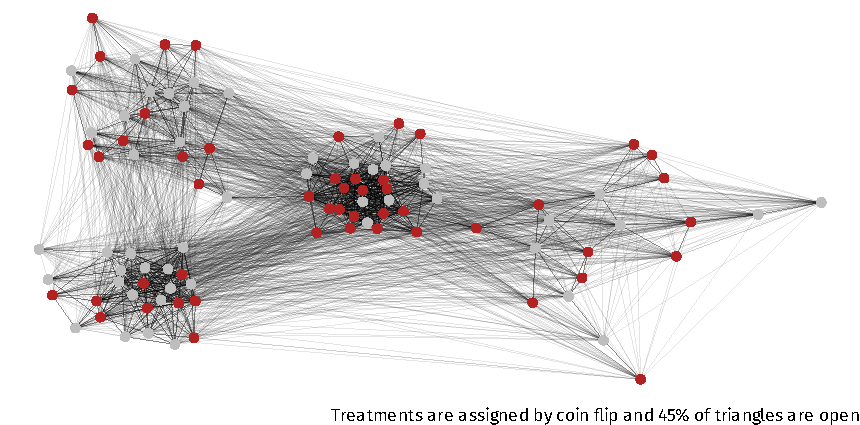
\includegraphics{./figures/simulations/jobtalk-backbone.pdf}
\end{frame}

\begin{frame}{...but we couldn't estimate peer effects!}
    It wasn't just us, none of the standard estimators worked!
    \begin{figure}
        \centering
        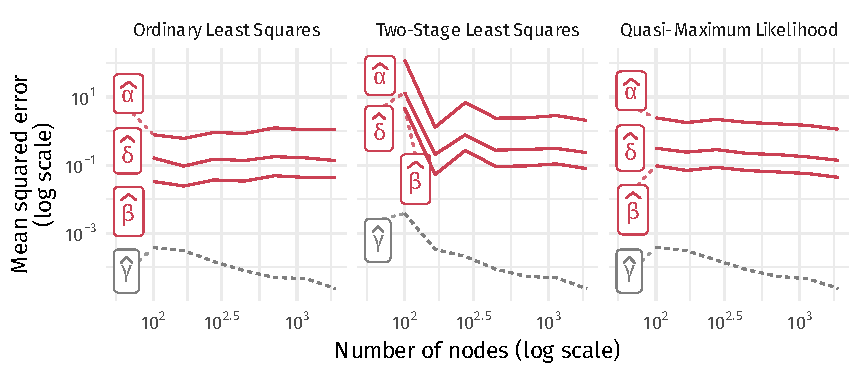
\includegraphics[width=\textwidth]{./figures/simulations/jobtalk-mse.pdf}
    \end{figure}
\end{frame}

\begin{frame}{The issue: the interference column converges to a constant in large samples}
    \centering
    \onslide<3->{
        When the network grows ($n \to \infty$),
    }
    \onslide<4->{
        if everyone makes more friends ($d_i \to \infty$)
    }
    \Large
    \vspace{6mm}
    \begin{equation*}
        \onslide<3->{
            \lim_{n \to \infty}
        }
        \onslide<1->{
            \underbrace{[GT]_i}_{\substack{\text{fraction} \\ \text{vaccinated} \\ \text{friends}}}
        }
        \onslide<2->{=}
        \onslide<3->{
            \lim_{n \to \infty}
        }
        \onslide<2->{
            \underbrace{
                \frac{1}{d_i} \sum_{j \, : \, A_{ij} = 1} T_j
            }_{\substack{\text{average of $d_i$}           \\ \text{i.i.d. coin flips}}}
        }
        \onslide<4->{
            = \frac 12   
        }
    \end{equation*} \\
    \normalsize
    \vspace{6mm}
    \onslide<5->{
        \underline{For every single node $i = 1, ..., n$}
    }
\end{frame}

\begin{frame}{Base rates and interence are collinear in large samples}
    \centering
    \begin{equation*}
        \begin{bmatrix}
            Y_1    \\
            Y_2    \\
            \vdots \\
            Y_n
        \end{bmatrix}
        =
        \underbrace{
            \begin{bNiceMatrix}[first-row,first-col]
                 & 1_n                     & GY     & T      & GT                        \\
                 & \textcolor{BrickRed}{1} & GY_1   & 1      & \textcolor{BrickRed}{1/2} \\
                 & \textcolor{BrickRed}{1} & GY_2   & 0      & \textcolor{BrickRed}{1/2} \\
                 & \vdots                  & \vdots & \vdots & \vdots                    \\
                 & \textcolor{BrickRed}{1} & GY_n   & 1      & \textcolor{BrickRed}{1/2}
            \end{bNiceMatrix}
        }_\text{as $n \to \infty$}
        \begin{bmatrix}
            \textcolor{BrickRed}{\alpha} \\
            \beta                        \\
            \gamma                       \\
            \textcolor{BrickRed}{\delta}
        \end{bmatrix}
        +
        \begin{bmatrix}
            \varepsilon_1 \\
            \varepsilon_2 \\
            \vdots        \\
            \varepsilon_n
        \end{bmatrix}
    \end{equation*} \\
    \vspace{8mm}
    \underline{Sometimes can't distinguish between base rate $\textcolor{BrickRed}{\alpha}$ and interference $\textcolor{BrickRed}{\delta}$}
\end{frame}

\begin{frame}{In simulations, we couldn't estimate $\textcolor{BrickRed}{\beta}$ either}
    \begin{figure}
        \centering
        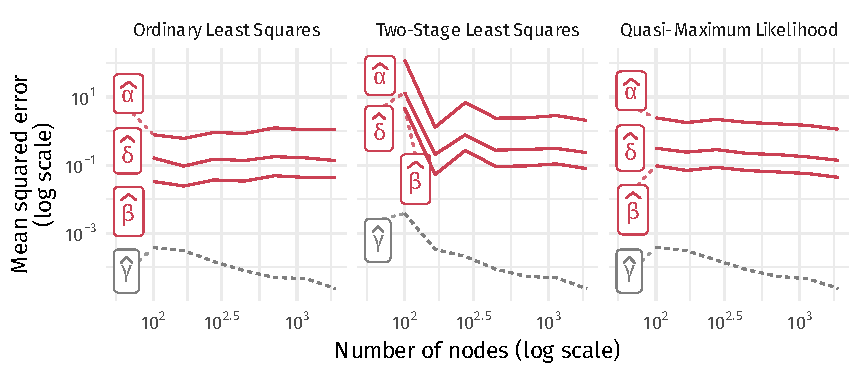
\includegraphics[width=\textwidth]{./figures/simulations/jobtalk-mse.pdf}
    \end{figure}
\end{frame}

\begin{frame}{Outcomes are generated by diffusing the treatment over the network}
    Why is $\textcolor{BrickRed}{\beta}$ also affected?
    \begin{align*}
        \onslide<1-> {
        Y             & = \alpha 1_n + \beta G Y + \gamma T + \delta G T + \varepsilon                        \\
        }
        \onslide<2-> {
        Y - \beta G Y & = \alpha 1_n  + \gamma T + \delta G T + \varepsilon                                   \\
        }
        \onslide<3->{
        Y             & = \paren*{I - \beta G}^{-1} \paren*{\alpha 1_n + \gamma T + \delta G T + \varepsilon} \\
        }
        \onslide<4->{
                      & \overset{*}{=} \underbrace{\sum_{k=0}^\infty \beta^k G^k}_{\substack{\text{repeated}  \\ \text{neighborhood} \\ \text{averaging}}} \paren*{\alpha 1_n + \gamma T + \delta G T + \varepsilon} \\
        }
    \end{align*}
    \footnotesize
    \onslide<4->{* Must have $\abs{\beta} < 1$, so effect of averaging decays with repetition}
\end{frame}

\begin{frame}{The contagion column converges to a constant in large samples}
    \begin{align*}
        GY = 
        \frac{\alpha}{1 - \beta} 1_n + 
        \underbrace{\gamma G T}_{\substack{\text{neighborhood}                                              \\ \text{average } \to \gamma / 2}} + 
        \underbrace{(\gamma \beta + \delta) \sum_{k=0}^\infty \beta^k G^{k+2} T}_{\substack{\text{repeated} \\ \text{neighborhood} \\ \text{averages} \\ \text{of $T$ *}}} +
        \underbrace{\sum_{k=0}^\infty \beta^k G^{k+1} \varepsilon}_{\substack{\text{repeated}               \\ \text{neighborhood} \\ \text{averages} \\ \text{of $\varepsilon$ } \to \, 0}}
    \end{align*} \\
    \vspace{4mm}
    Each term in the sum converges to a constant
    \begin{align*}
        GY & \to \eta
    \end{align*} \\
    \vspace{4mm}
    \footnotesize
    * Neighborhood average of a constant is that same constant
\end{frame}

\begin{frame}{Base rates, interference and contagion are collinear in large samples}
    
    \begin{equation*}
        \begin{bmatrix}
            Y_1    \\
            Y_2    \\
            \vdots \\
            Y_n
        \end{bmatrix}
        =
        \underbrace{
            \begin{bNiceMatrix}[first-row,first-col]
                 & 1_n                     & GY                         & T      & GT                        \\
                 & \textcolor{BrickRed}{1} & \textcolor{BrickRed}{\eta} & 1      & \textcolor{BrickRed}{1/2} \\
                 & \textcolor{BrickRed}{1} & \textcolor{BrickRed}{\eta} & 0      & \textcolor{BrickRed}{1/2} \\
                 & \vdots                  & \vdots                     & \vdots & \vdots                    \\
                 & \textcolor{BrickRed}{1} & \textcolor{BrickRed}{\eta} & 1      & \textcolor{BrickRed}{1/2}
            \end{bNiceMatrix}
        }_\text{as $n \to \infty$}
        \begin{bmatrix}
            \textcolor{BrickRed}{\alpha} \\
            \textcolor{BrickRed}{\beta}  \\
            \gamma                       \\
            \textcolor{BrickRed}{\delta}
        \end{bmatrix}
        +
        \begin{bmatrix}
            \varepsilon_1 \\
            \varepsilon_2 \\
            \vdots        \\
            \varepsilon_n
        \end{bmatrix}
    \end{equation*} \\
    \vspace{6mm}
    \begin{center}
        \underline{Sometimes can't distinguish between base rate $\textcolor{BrickRed}{\alpha}$, interference $\textcolor{BrickRed}{\delta}$ and contagion $\textcolor{BrickRed}{\beta}$} \\
    \end{center}
\end{frame}

\begin{frame}{Peer effects are asymptotically collinear under very general circumstances}
    \begin{assumption}
        \begin{enumerate}
            \item $T_1,T_2,\dots,T_n$ are independent with shared mean $\tau \in \R$, and $T$ is independent of $A$.
            \item $\{ T_i - \tau : i \in [n] \}$ are independent subgamma random variables.
            \item $\varepsilon_1, \varepsilon_2, \dots, \varepsilon_n$ are independent subgamma random variables.
            \item The minimum degree grows strictly faster than $\log n$, such that
                  \begin{equation*}
                      \lim_{n \to \infty} \frac{\min_{i \in [n]} d_i}{\log n} = \infty.
                  \end{equation*}
        \end{enumerate}
    \end{assumption}
    
    Recall: 
    \Large
    \begin{equation*}
        Y = \alpha 1_n + \beta G Y + T \gamma + G T \delta + \varepsilon
    \end{equation*}
\end{frame}

\begin{frame}{These assumptions are distributionally agnostic}
    \begin{definition}[\citealt{boucheron2013}]
        Let $Z$ be a mean-zero random variable with cumulant generating function $\psi_Z(t) = \log \E{e^{t Z}}$.
        $Z$ is \emph{subgamma} with parameters $\nu \ge 0$ and $b \ge 0$ if
        \begin{equation*}
            \psi_Z(t) \le \frac{t^2 \nu}{2 (1 - b t)}
            ~\text{ and }~
            \psi_{-Z}(t) \le \frac{t^2 \nu}{2 (1 - b t)}
            ~\text{ for all }~ t < 1 / b.
        \end{equation*}
        We then write that $Z$ is $(\nu,b)$-subgamma.
    \end{definition}
    \vspace{4mm}
    \underline{Examples}: Bernoulli, Poisson, Exponential, Gamma, Gaussian, sub-Gaussian, squared sub-Gaussians, bounded distributions, etc
\end{frame}

\begin{frame}{The interference and contagion columns converge uniformly to constants}
    
    \begin{lemma}
        Under the previous assumptions,
        \begin{equation*}
            \max_{i \in [n]} \Big| [GT]_i - \tau \Big|
            = o(1) ~ \text{ almost surely }
        \end{equation*}
        and there exists $\eta \in \R$ such that
        \begin{equation*}
            \max_{i \in [n]} \Big| [GY]_i - \eta \Big|
            = o(1) ~ \text{ almost surely.}
        \end{equation*}
    \end{lemma}
\end{frame}

\begin{frame}{Collinearity shows up quickly in finite samples}
    \vspace{3mm}
    \centering
    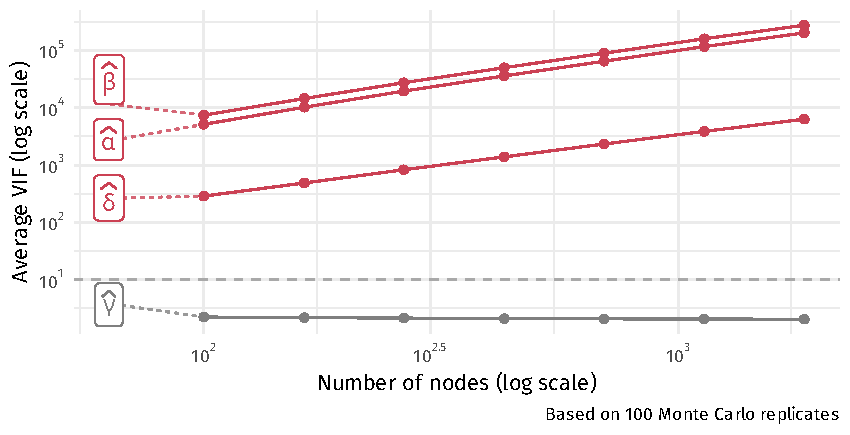
\includegraphics{./figures/simulations/defense-vif.pdf}
\end{frame}

\begin{frame}{Asymptotic collinearity can lead to inconsistency}
    \begin{theorem}[\citealt{hayes2024c}]
        Let $(\alphahat, \betahat, \gammahat, \deltahat)$ be the vector of ordinary least squares estimates of $(\alpha, \beta, \gamma, \delta)$. Recall that $G = D^{-1} A$ is the row-normalized adjacency matrix. Suppose that the degrees of the network are such that $\| G \|_F^2 = o(n)$.
        Then if $\beta = 0$,
        \begin{equation*}
            \min\{ |\alphahat-\alpha|, |\betahat-\beta| \}
            = \Omegap{ 1 }
        \end{equation*}
        and
        \begin{equation} \label{eq:deltahat:LB}
            | \deltahat - \delta | = \Omegap{ \frac{1}{\|G\|_F} }.
        \end{equation}
        If $\beta \neq 0$,
        \begin{equation*}
            \min\{ |\alphahat-\alpha|, |\betahat-\beta| \}
            = \Omegap{ \frac{1}{\|G\|_F} }.
        \end{equation*}
        Under the stronger assumption $\|G\|_F^2 = o( \sqrt{n} )$, eq.~\eqref{eq:deltahat:LB} holds for all $\beta$.
    \end{theorem}
\end{frame}


\begin{frame}{Asymptotic collinearity can lead to inconsistency}
    \begin{theorem}[Intuitive]
        When minimum degree grows, ordinary least squares estimates of $\alpha, \beta$ and $\delta$ are either inconsistent, or at best consistent at $\sqrt{n / d_{\min}}$ rates, where $d_{\min} = \min_{i \in [n]} d_i$.
    \end{theorem}
    
    This is because the \textcolor{BrickRed}{signal-to-noise ratio} depends on the minimum degree\footnote{Our lower bound matches the upper bound on estimation error in \cite{lee2004}.}.
\end{frame}

\begin{frame}{\textcolor{BrickRed}{Asymptotic collinearity} affects other estimators as well}
    \vspace{3mm}
    \centering
    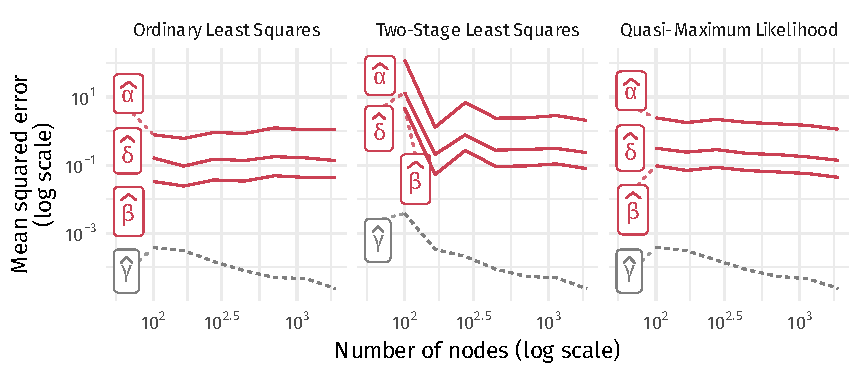
\includegraphics{./figures/simulations/jobtalk-mse.pdf}
\end{frame}

\begin{frame}{Details: weighted and directed networks}
    \textbf{Weighted networks}: If $A \in \R^{n \times n}_{\ge 0}$ is a positive, weighted network with $(\nu, b)$-subgamma edges $A_{ij}$, we require that
    \begin{equation*}
        \max_{i \in [n]} \frac{1}{d_i^2} \sum_{j=1}^n A_{ij}^2
        = o\left( \frac{ 1 }{ \nu \log^2 n } \right)
        ~\text{ and }~
        \max_{j \in [n]} \frac{ A_{ij} }{ d_i }
        = o\left( \frac{ 1 }{ b \log n } \right).
    \end{equation*} \\
    Roughly: no one edge can be too important for a given node \\
    \vspace{4mm}
    \textbf{Directed networks}: extension possible, but slightly more involved \\
    \vspace{4mm}
    \textbf{Isolated nodes}: can allow a vanishing fraction of nodes to be isolated
\end{frame}


\begin{frame}
    \textbf{Standard wisdom} states that collinearity isn't a problem in linear-in-means in networks with open triangles.
    
    \vspace{4mm}
    
    \begin{block}{Takeaway 1}
        When nodal covariates are independent of the network, we show that peer effects may not be estimable, due to collinearity, even when there are many open triangles.
    \end{block}
    
    \vspace{4mm}
    
    \begin{block}{Takeaway 2}
        Direct effects are estimable even when there is asymptotic collinearity.
    \end{block}
\end{frame}

\begin{frame}{Why hasn't the spatial econometrics literature encountered this issue before?}
    
    \begin{enumerate}
        \item Often treat covariates $T$ and network $G$ as fixed rather than random
        \item Theory directly assumes there is no asymptotic collinearity
        \item Simulations rarely investigate consistency of estimators
    \end{enumerate}
    % \vspace{4mm}
    % More recent causal work has explicitly leveraged asymptotic collinearity in random graphs to estimate direct effects \citep{li2022f}
\end{frame}

\begin{frame}{The interference literature is well-aware of issues with Bernoulli designs}
    \vfill
    \begin{columns}
        \begin{column}{0.5\textwidth}
            \centering
            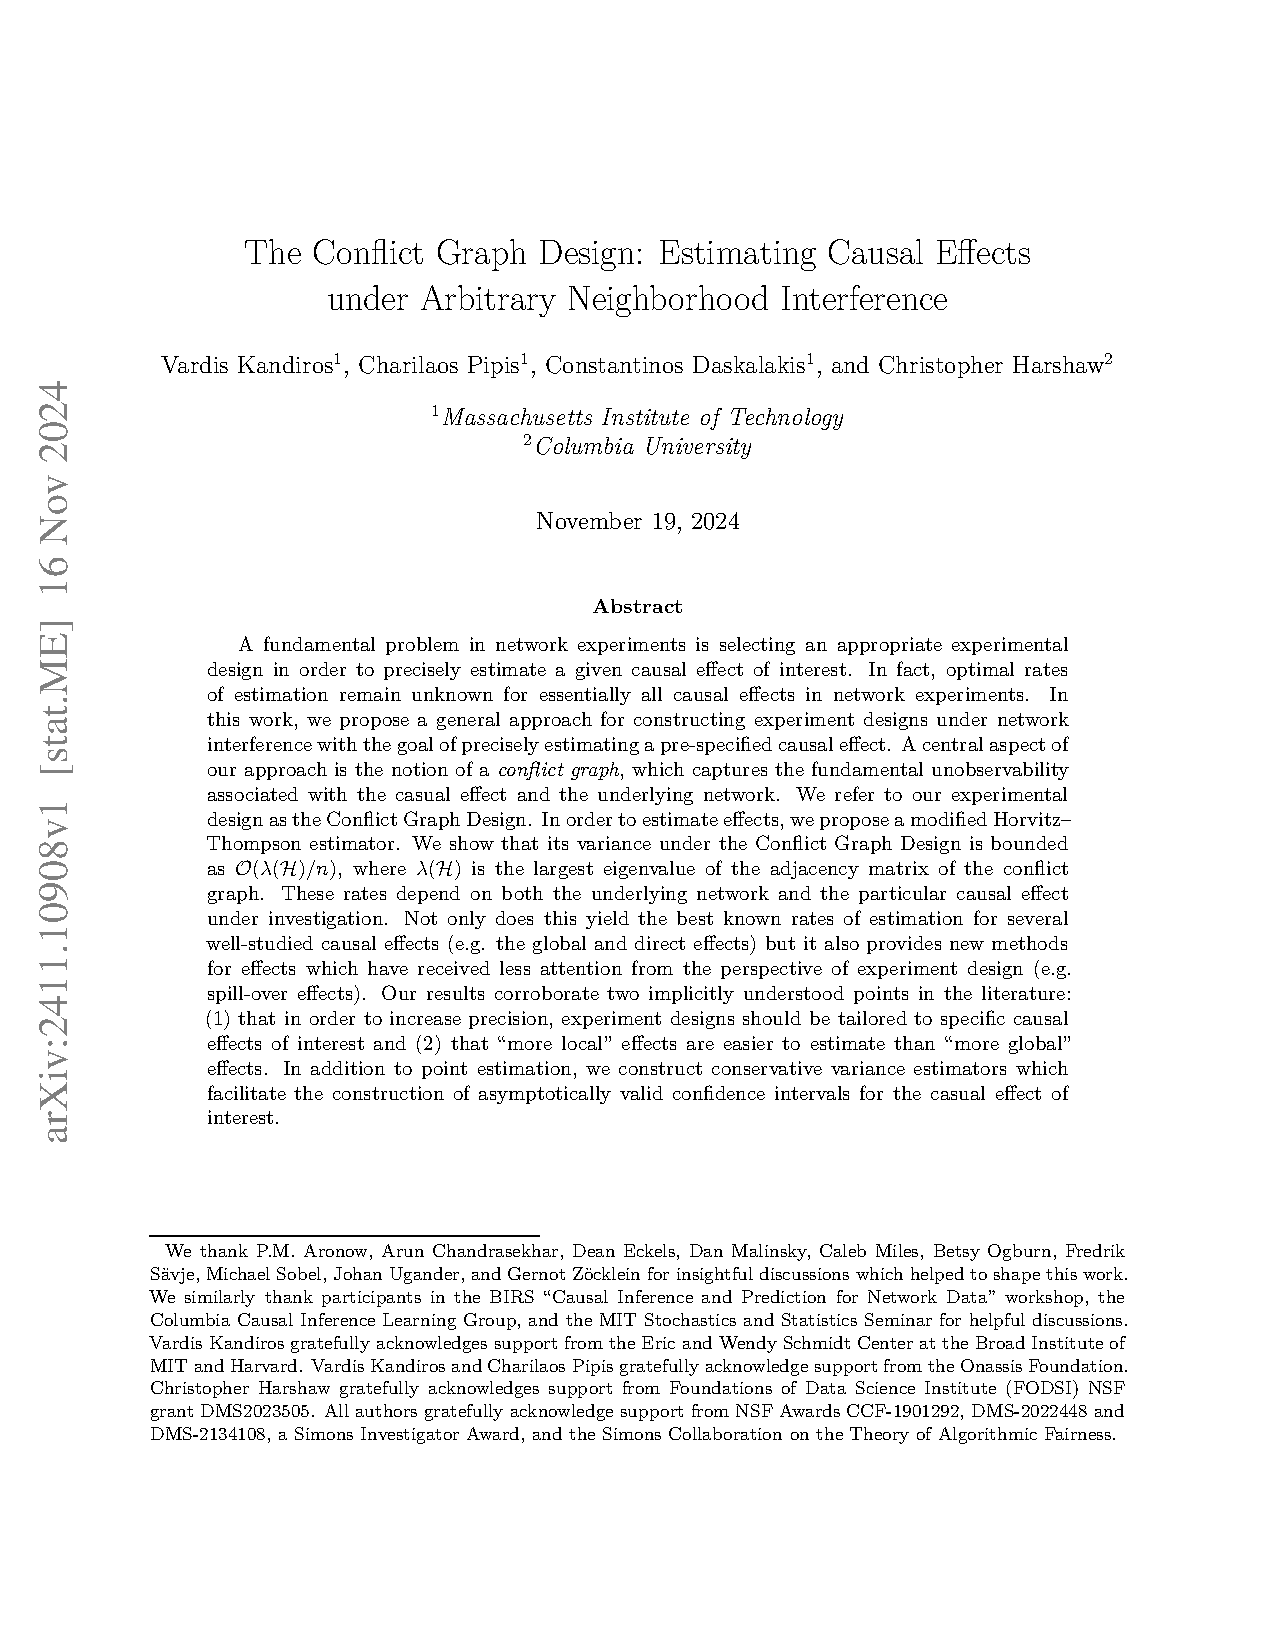
\includegraphics[height=0.95\textheight, page=1, trim={2.5cm 8cm 0 2cm}, clip]{./papers/conflict.pdf}
        \end{column}
        \begin{column}{0.5\textwidth}
            \centering
            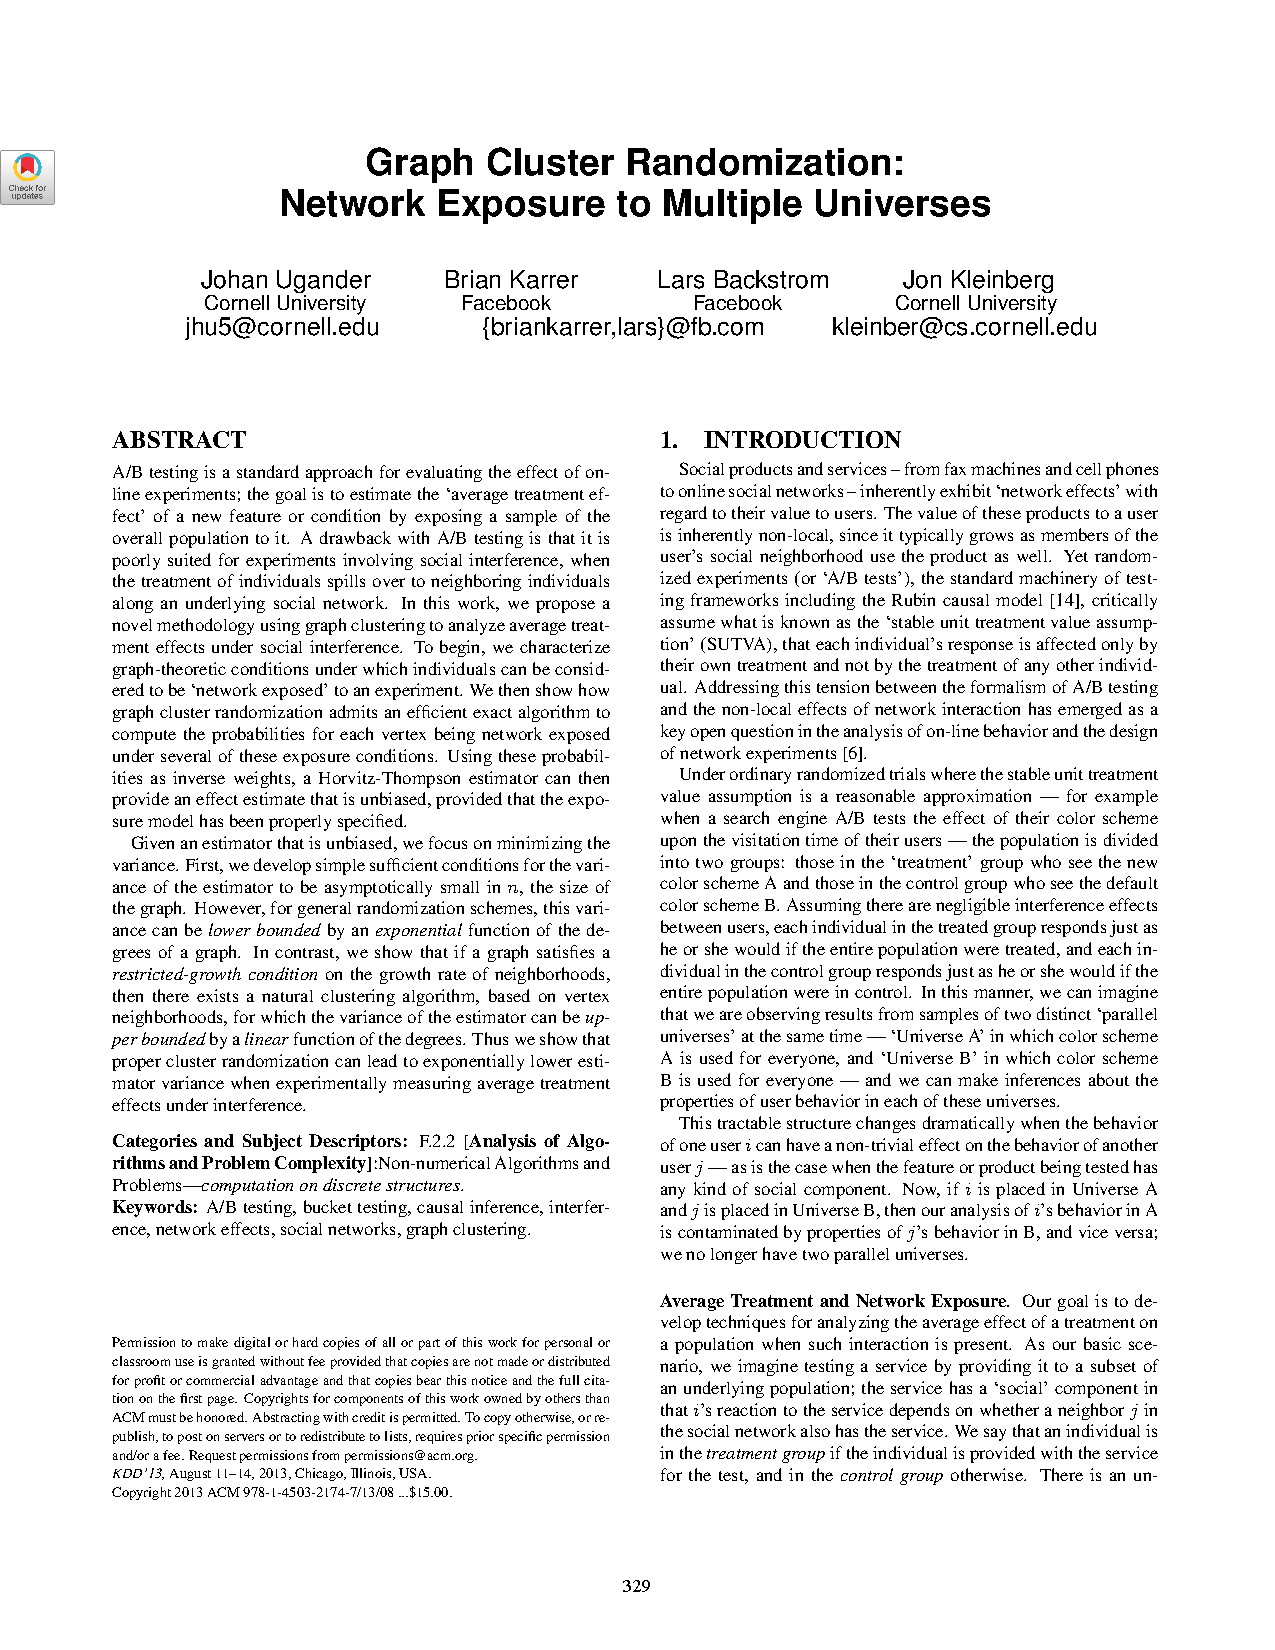
\includegraphics[width=\textwidth, page=1, trim={1.5cm 9cm 0 2.5cm}, clip]{./papers/gcr.pdf}
        \end{column}
    \end{columns}
\end{frame}

\begin{frame}{Causal folks are interested in treatments that depend on position in network}
    \centering
    \includegraphics[width=\textwidth, page=2, trim={1.5cm 16cm 0 3.3cm}, clip]{./papers/shalizi.pdf}
\end{frame}

\begin{frame}{Dependence between treatment and network might resolve collinearity issues}
    \Large
    \begin{align*}
        \underbrace{[GT]_i}_{\substack{\text{fraction} \\ \text{vaccinated} \\ \text{friends}}}
        = \underbrace{
            \frac{1}{d_i} \sum_{j \, : \, A_{ij} = 1} T_j
        }_{\substack{\text{average of dependent treatments}}}
    \end{align*} \\
    \normalsize
    \centering
    \vspace{8mm}
    $GT$ might not converge, or might converge to non-constant value
\end{frame}

\begin{frame}{We considered models where treatment depended on position in network}
    \centering
    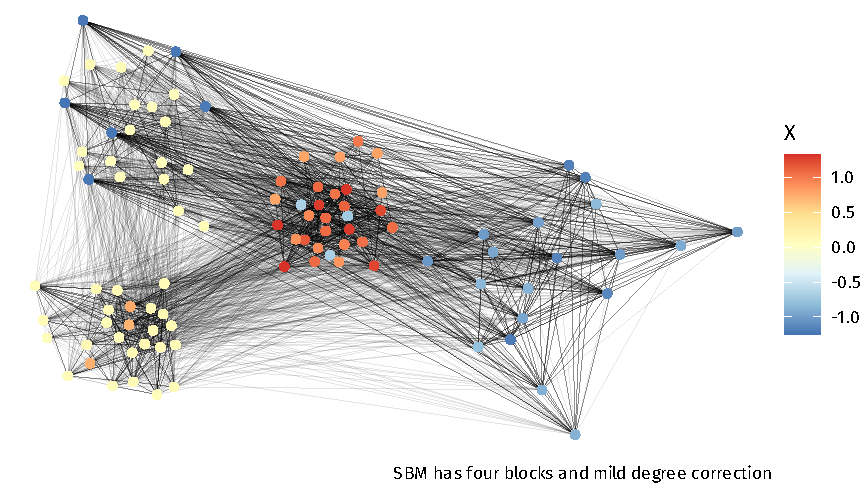
\includegraphics{./figures/simulations/defense-backbone-dependent.pdf}
\end{frame}

\begin{frame}{We considered models where treatment depended on position in network}
    
    \begin{columns}
        \column{0.45\textwidth}
        \centering
        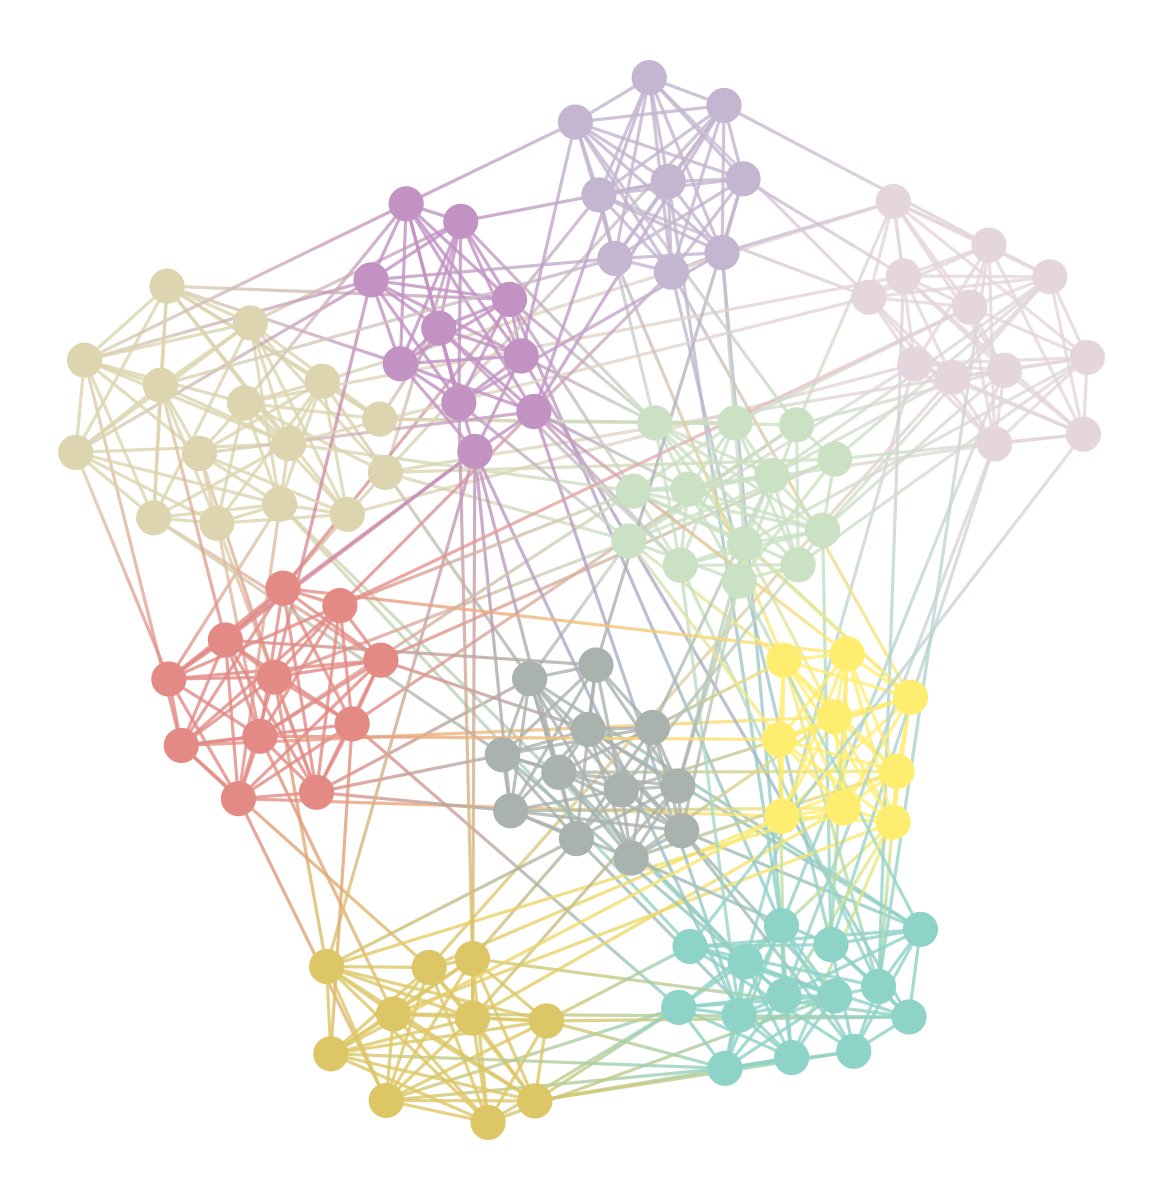
\includegraphics[width=\textwidth]{./figures/assortative.png}
        \column{0.55\textwidth}
        
        Stochastic blockmodels are an intuitive way to induce dependence \\
        \vspace{4mm}
        
        Block indicators $Z_i$ \\
        Popularity parameters $\theta_i$ \\
        Mixing matrix $B \in [0, 1]^{d \times d}$
        
        \begin{equation*}
            \mathbb P[Z, \theta]{A_{ij} = 1} = \theta_i Z_i B Z_j^T \theta_j
        \end{equation*}
    \end{columns}
\end{frame}

\begin{frame}{Linear-in-means models on blockmodels are of independent interest!}
    \centering
    
\includegraphics[height=0.95\textheight, page=1, trim={1.5cm 6cm 0 4cm}, clip]{./papers/paul.pdf}
\end{frame}

\begin{frame}{We prove a partial asymptotic collinearity result for these models}
    \begin{theorem}[\citealt{hayes2024c}]
        Suppose that $A$ is sampled from a degree-corrected stochastic blockmodel. Define $X_i = \theta_i Z_i$. Let 
        \begin{equation*}
            Y = \alpha 1_n + \beta G Y + X \gamma + G X \delta + \varepsilon
        \end{equation*}
        for $\alpha, \beta \in \R$ and $\gamma, \delta \in \R^d$. Suppose that $X$ has $k \ge 2d$ distinct rows. Then, under some conditions,
        \begin{equation*}
            W_n = \begin{bmatrix}
                1_n & GY & X & GX
            \end{bmatrix}
        \end{equation*}
        converges uniformly to a limit object with rank $2d$ out of $2d + 2$. If any two entries of $(\alpha, \beta, \delta_1, ..., \delta_d)$ are set to zero in the data generating process, the limit object of $W_n$ is a matrix with full rank.
    \end{theorem}
\end{frame}

\begin{frame}{We prove a partial asymptotic collinearity result for these models}
    \textbf{Key condition to avoid collinearity}: sufficient degree heterogeneity such that $X$ and $D^{-1} X$ are linearly independent
    
    \vspace{4mm}
    \textbf{General low-rank networks}: if $\mathbb E[ A_{ij} \mid X ] = X_i^T X_j$, a similar result holds, broadly generalizing the partial identification result
    
    \vspace{4mm}
    Explains \textcolor{BrickRed}{counterintuitive} simulations in \cite{paul2022}; had to drop intercept column to avoid asymptotic collinearity!
\end{frame}

\begin{frame}{We performed a simulation study to confirm the theoretical results}
    \begin{itemize}
        \setlength\itemsep{1.75em}
        \item \textcolor{BrickRed}{Bernoulli}: Treatment random and independent of network. $T_i \diid \Bern(0.5)$
              \begin{equation*}
                  Y = \textcolor{BrickRed}{\alpha} 1_n + \textcolor{BrickRed}{\beta} G Y + T \gamma + G T \textcolor{BrickRed}{\delta} + \varepsilon,
              \end{equation*}
              with $\textcolor{BrickRed}{\alpha} = 3, \textcolor{BrickRed}{\beta} = 0.2, \gamma = 4, \textcolor{BrickRed}{\delta} = 2$ and $\varepsilon \diid \calN(0, \sigma^2)$ with $\sigma = 0.1$.
        \item \textcolor{BrickRed}{Unrestricted model}: Treatment random and dependent on network. Define $X_i = \theta_i Z_i \in \R^4$
              \begin{equation*}
                  Y = \textcolor{BrickRed}{\alpha} 1_n + \textcolor{BrickRed}{\beta} G Y + X \gamma + G X \textcolor{BrickRed}{\delta} + \varepsilon,
              \end{equation*}
              where $\textcolor{BrickRed}{\alpha} = 3, \textcolor{BrickRed}{\beta} = 0.2$ and $\varepsilon \diid \calN(0, \sigma^2)$ with $\sigma = 0.1$. Since $X_i \in \R^4$, $\gamma, \textcolor{BrickRed}{\delta} \in \R^4$ and we fix $\textcolor{BrickRed}{\delta} = (2, 2, 2, 2)$ and $\gamma = (1.5, 2.5, 3.5, 4.5)$.
        \item Restricted model: The unrestricted model, but $\delta = (0, 0, 2, 2)$, so there's no asymptotic collinearity.
    \end{itemize}
\end{frame}

\begin{frame}{Dependence prevented \textcolor{BrickRed}{asymptotic collinearity} and estimation challenges}
    \centering
    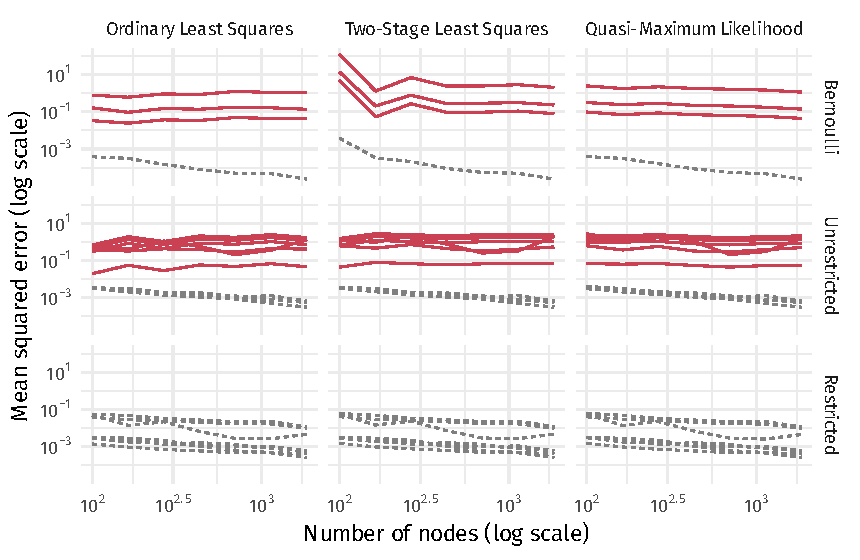
\includegraphics[width=0.85\textwidth]{./figures/simulations/jobtalk-mse-all.pdf}
\end{frame}

\begin{frame}

    \begin{block}{Takeaway 3}
        Explicitly modelling dependence between nodal covariates and network structure can aid identifiability and resolve asymptotic collinearity issues.
    \end{block}
    \vspace{4mm}
    \begin{block}{Takeaway 4}
        Treatments dependent on network must be considered on a case-by-case basis, considering both the treatment and the network model.
    \end{block}
\end{frame}


\begin{frame}{Open questions about linear-in-means models}
    
    Is asymptotic collinearity an issue in \textbf{longitudinal models} of peer effects like \cite{zhu2017, mcfowland2021, katsouris2024}? \\
    \vspace{8mm}
    Can asymptotic collinearity be avoided via additional assumptions on the \textbf{error covariance} $\varepsilon$, as in \cite{rose2017}? 
\end{frame}

\begin{frame}{Thank you! Questions?}
    \footnotesize \phantom{test} \normalsize
    \begin{columns}
        \begin{column}{0.4\textwidth}
            \begin{itemize}
                \item[] \faIcon[regular]{envelope} \href{mailto:alex.hayes@wisc.edu}{alex.hayes@wisc.edu}
                \item[] \faIcon{wordpress} \href{https://www.alexpghayes.com}{alexpghayes.com}
                \item[] \faIcon{github} \href{https://github.com/alexpghayes}{github.com/alexpghayes}
            \end{itemize}
        \end{column}
        \begin{column}{0.6\textwidth}
            \centering
            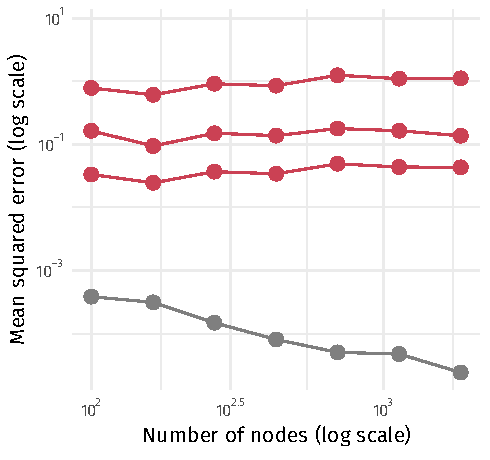
\includegraphics[scale=0.65]{./figures/simulations/jobtalk-last-slide.pdf}
        \end{column}
    \end{columns}
    \footnotesize
    \begin{block}{Pre-print}
        Alex Hayes and Keith Levin. “Peer Effects in the Linear-in-Means Model May Be Inestimable Even When Identified.” arXiv, October 14, 2024. \url{http://arxiv.org/abs/2410.10772}.
    \end{block}
\end{frame}

\appendix


\begin{frame}{A formal definition for identifiability}
    \begin{definition}[\citealt{maclaren2020a}]
        A model $\mathcal M = \{ P_\theta : \theta \in \Theta \}$ is a collection of probability measures $P_\theta$, indexed by a set $\Theta$. A parameter $q(\theta)$ is \emph{identifiable} if and only if $q(\theta_1) \neq q(\theta_2)$ implies $P_{\theta_1} \neq P_{\theta_2}$.
    \end{definition}
\end{frame}

\begin{frame}{Several equivalent conditions for identifiability in linear models}
    In linear models, where $Y_i = X_i \theta + \varepsilon_i$ and $\varepsilon_i \sim \mathcal N(0, \sigma^2)$, the following are equivalent \citep{lewbel2019}:
    \begin{enumerate}
        \item $\theta$ is identified
        \item $X$ is full-rank (i.e., there is no perfect collinearity)
        \item the covariance matrix $X^T X / n$ is full-rank
        \item the log-likelihood
              \[
                  -\frac{n}{2}\log(2\pi\sigma^2) - \frac{1}{2\sigma^2}\sum_{i=1}^n(y_i - x_i\theta)^2
              \]
              has a unique maximizer.
    \end{enumerate}
\end{frame}


\begin{frame}{A linear model that is identified, asymptotically collinear, and inestimable}
    
    Suppose that all data points except for the first data point are exactly equal:
    
    \begin{equation*}
        \begin{bmatrix}
            Y_1    \\
            Y_2    \\
            Y_3    \\
            \vdots \\
            Y_n
        \end{bmatrix}
        =
        \begin{bmatrix}
             & 1      & 2      &   \\
             & 1      & 1      &   \\
             & 1      & 1      &   \\
             & \vdots & \vdots &   \\
             & 1      & 1      & 
        \end{bmatrix}
        \begin{bmatrix}
            \alpha \\
            \beta
        \end{bmatrix}
        +
        \begin{bmatrix}
            \varepsilon_1 \\
            \varepsilon_2 \\
            \varepsilon_3 \\
            \vdots        \\
            \varepsilon_n
        \end{bmatrix}
    \end{equation*}
    Then $\alpha$ and $\beta$ are identified but cannot be estimated
\end{frame}

\begin{frame}
    \underline{Estimators}
    \begin{itemize}
        \setlength\itemsep{1.25em}
        \item OLS: \texttt{lm($y \sim Gy + T + GT$)}
        \item TSLS: \texttt{ivreg}($y \sim Gy + T + GT \mid \underbrace{T + GT + G^2T}_\text{instruments}$)
    \end{itemize}
\end{frame}


\begin{frame}

    \begin{definition}[Random Dot Product Graph, \citealt{young2007}]
        Let $F$ be a distribution on $\R^d$ such that $0 \le x^T y$ for all $x,y \in \supp F$ and the convex cone of $\supp F$ is $d$-dimensional.
        Draw $X_1,X_2,\dots,X_n \diid F$, and collect these in the rows of $X \in \R^{n \times d}$ for ease of notation.
        Conditional on these $n$ vectors, which we call {\em latent positions}, generate edges by drawing the edges $\{ A_{ij} : 1 \le i < j \le n \}$ as independent $(\nu,b)$-subgamma random variables with $\mathbb E[ A_{ij} \mid X ] = \rho X_i^T X_j$, where $\rho \in [0,1]$.
        Then we say that $A$ is distributed according to an $n$-vertex random dot product graph with latent position distribution $F$, $(\nu,b)$-subgamma edges and sparsity factor $\rho$.
        We write $(A,X) \sim \RDPG( F, n)$, with the subgamma and sparsity parameters made clear from the context.
    \end{definition}
\end{frame}

\begin{frame}
    \begin{proposition}
        \label{prop:XHX-rank}
        Let $\mu = \E{X} \in \R^d$ and suppose that $Y_1,Y_2,\dots,Y_d,Z_1,Z_2,\dots,Z_d \in \R^d$ are rows of $X \in \R^{n \times d}$ such that $Y_1,Y_2,\dots,Y_d$ are linearly independent and $Z_1,Z_2,\dots,Z_d$ are linearly independent.
        \begin{equation*}
            H_Y = \diag\left( Y_1^T \mu, Y_2^T \mu, \dots, Y_d^T \mu \right)
            ~~~\text{ and }~~~
            H_Z = \diag\left( Z_1^T \mu, Z_2^T \mu, \dots, Z_d^T \mu \right).
        \end{equation*}
        Provided that $Z^{-1} H_Z^{-1} Z - Y^{-1} H_Y^{-1} Y \in \R^{d \times d}$ is invertible, then the matrix
        \begin{equation*} \label{eq:targetmx}
            M = \begin{bmatrix} X & H^{-1} X \end{bmatrix} \in \R^{n \times 2d}
        \end{equation*}
        has rank $2d$.
    \end{proposition}
    
    \underline{Morally:} need degree heterogeneity so that $X$ and $D^{-1} X$ are linearly independent
\end{frame}

\begin{frame}
    \underline{Technical conditions for partial identification result} \\
    \vspace{6mm}
    \begin{itemize}
        \setlength{\itemsep}{1.75em}
        \item $\rho = \omega \left( \displaystyle \frac{ \log^2 n }{ \sqrt{n} } \right)$ and $\displaystyle \frac{ \nu + b^2 }{ \rho } = \Theta( 1 )$
        \item $\displaystyle \min_{i \in [n]} \abs*{X_i^T \, \E{X_1}} = \omega\left( \frac{ \log^2 n }{ \sqrt{ n } \rho } \right)$ almost surely.
        \item $\displaystyle \max_{i \in [n]} \| X_i \| = o(\sqrt{n})$ almost surely.
        \item $\displaystyle \mathbb E \| X_1 \|^2 < \infty$.
    \end{itemize}
\end{frame}

\bibliographystyle{chicago}
\bibliography{2025-02-19-jobtalk}

\end{document}